\chapter{Introduction} \label{sec:Introduction}
Optimizing predictive models on datasets obtained from citizen-science projects can be computationally expensive as these datasets grow in size. Consequently, running models based on Multi-layered Neural Networks, Integer Programming and other optimization routines can become more computationally difficult as the number of parameters increase, despite using the faster Central Processing Units (CPUs) in the market. Incidentally, it becomes difficult for citizen-science projects, which often deal with large datasets, to scale if the organizers do not employ special processing units to run neural networks as optimization models, which require extensive tensor operations. One such special processing unit is the Graphical Processing Units (GPUs), which offer numerous cores to parallelize computation. These can often outperform CPUs in computing such predictive models if these models \textit{heavily} rely on large-scale tensor operations \cite{ParallelNVIDIA, cuDNNPaper}. By using GPUs over CPUs to accelerate computation on a citizen-science project, the model could achieve better optimization in less time, enabling the project to scale.

\section{Avicaching} \label{sec:Avicaching}
Part of the eBird project, which aims to ``maximize the utility and accessibility of the vast numbers of bird observations made each year by recreational and professional bird watchers'' \cite{EBird}, Avicaching is a incentive-driven game trying to homogenize the spatial distribution of citizens' (agents') observations \cite{Xue2016Avi1, Xue2016Avi2}. Since the dataset of agents' observations in eBird is geographically heterogeneous (concentrated in some places like cities and sparse in others), Avicaching homogenizes the observation set by placing rewards at and attracting agents to under-sampled locations \cite{Xue2016Avi1}. For the agents, collecting rewards increases their `utility' (excitement, fun etc.), while for the organizers, a more homogeneous observation dataset means better sampling and higher confidence in using it for other models. 
\begin{figure}[!htbp]
    \centering
    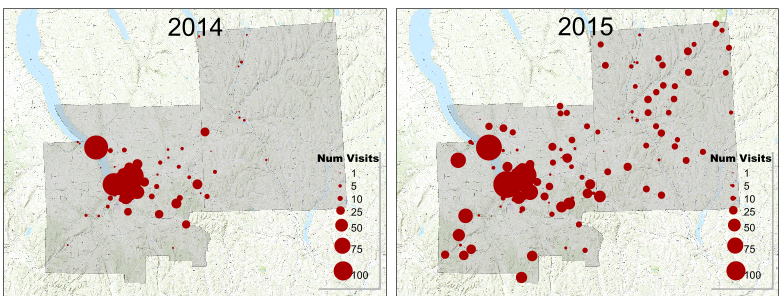
\includegraphics[width=\textwidth]{avicaching_change}
    \caption[Avicaching 2014-15 Results in Tompkins and Cortland Counties]{Avicaching 2014-15 Results in Tompkins and Cortland Counties, NY: With the previous model \cite{Xue2016Avi1, Xue2016Avi2, EBird}, Avicaching was able to attract `eBirders' to under-sampled locations by distributing rewards over the location set.}
    \label{fig:Avicaching 2014-15 Results in Tompkins and Cortland Counties}
\end{figure}

To accomplish this task of specifying rewards at different locations based on the historical records of observations, Avicaching would learn how agents change their behavior when a certain sample of rewards were applied to the set of locations, and then redistribute rewards across the locations based on those learned parameters \cite{Xue2016Avi2}. This requirement naturally translates into a  optimization problem, implemented using multi-layered neural networks and linear programming.

\section{Important Questions} \label{sec:Important Questions}
Although the previously devised solutions to Avicaching were conceptually effective \cite{Xue2016Avi1, Xue2016Avi2}, using CPUs to solve Mixed Integer Programming and (even) shallow neural networks made the models impractical to scale. Solving the problems faster would have also allowed organizers to find better results (more optimized). These concerns, which form the pivot for our research, are concisely described below.

\subsection{Solving Faster} \label{sec:Important Questions - Solving Faster}
We were interested in using GPUs to run our optimization models because of their capability to accelerate problems based on large tensor operations \cite{ParallelNVIDIA, cuDNNPaper}. Newer generation NVIDIA GPUs, equipped with thousands of CUDA (NVIDIA's parallel computing API) cores \cite{NVIDIA}, could have empowered Avicaching's organizers to scale the game, if the underlying models were computed using simple arithmetic operations on tensors, rather than using conditional logic (see \Cref{sec:Avoiding Specific Operations in GPUs}). Since even the faster CPUs - in the range of Intel Core i7 chipsets - are sequential in processing and do not provide as comparable parallel processing\footnote{CPUs often have multiple cores nowadays, but very few compared to what many GPUs have.} as GPUs do, we sought to solve the problem much faster using GPUs. But \textbf{how fast could we do it?}

\subsection{Better Results} \label{sec:Important Questions - Better Results}
The previously devised sub-model for learning parameters in agents' change of behavior on a fixed set of rewards delivered predictions that differed $26\%$ from Ground Truth \cite[Table 1]{Xue2016Avi2}. This model was then used to redistribute rewards in a budget. If we could get closer to the Ground Truth, i.e., better learn the parameters for the change, we could redistribute rewards with superior prediction/accuracy. Since the organizers require the \textit{best} distribution of rewards, we will need a set of learned parameters that is closer to the Ground Truth (in terms of Normalized Mean Squared Error \cite[Section 4.2]{Xue2016Avi2}). In a gist, we aimed to \textbf{learn the parameters more suitably}, and \textbf{find the  best allocation of rewards.}

\subsection{Adjusting the Model's Features} \label{sec:Important Questions - Adjusting the Model's Features}
Once the model starts delivering better results than the previously devised models, one thinks if some characteristics\footnote{Tinkering with hyper-parameters like learning rate or adding a weight regularizer.} of the model can be changed to get more preferable results (one could also build a better model). While a goal of ``getting better results'' is an unending struggle, there is a trade-off with practicality as these adjustments take time and computation power to test - and we didn't have unlimited resources. Therefore, we asked if one could \textbf{reasonably adjust the model's features to improve performance and optimization.}

\section{Computation Using GPUs} \label{sec:Computation Using GPUs}
The use of GPUs has changed drastically in the last decade - from rendering superior graphics to parallelizing floating point operations. Companies like NVIDIA are now providing General Purpose GPUs (GPGPUs) that are capable of executing parallel algorithms using thousands of cores and threads \cite{NVIDIA}. Furthermore, by working with newly-developed parallel programming APIs like CUDA, one can handle a GPU's threads more efficiently and optimize an task's datapath \cite{CUDADocs}. In the next sections, we briefly describe NVIDIA GPU's architecture, instruction set and best practices for optimization. Although we do not implement the CUDA back-end manually and use PyTorch's implementation \cite{PTDocs}, understanding the basics of the processor can be helpful for designing our models.

\subsection{GPU Architecture} \label{sec:GPU Architecture}
We describe the structure and abstractions of an NVIDIA GPU with Pascal architecture\footnote{We use NVIDIA Quadro P4000 (Pascal architecture) for our tests.}. These devices are multi-threaded multi-processors for executing ``fine-grained threads efficiently'' \cite[Appendix~B.4]{PattersonARM}. Unlike Personal Computer CPUs, which currently comprise 1-8 cores with fast and low-latency datapath, GPUs provide scalable parallel processing power with high throughput and latency\footnote{High latency is undesirable.} \cite{PattersonARM, DemystifyingGPU}. Informally, GPUs are often referred to as a collection of many `dumb' cores, unlike the few `smart' cores in a CPU. Nonetheless, GPUs are efficient in executing simple instructions in parallel, using hierarchies of cores, threads and memory.

\subsubsection{Core Organization}
In most architectures by NVIDIA, many Scalar Processors (SP or CUDA cores) are clustered in a Streaming Multiprocessor (SM), which are then organized in Grid Processing Clusters (GPCs). A GPU can have several GPCs, as shown in \Cref{fig:Organization of Cores in NVIDIA Pascal GP100 GPU} \cite{CUDADocs,ParallelNVIDIA,DemystifyingGPU}.
\begin{figure}
    \centering
    \begin{subfigure}{\textwidth}
        \centering
        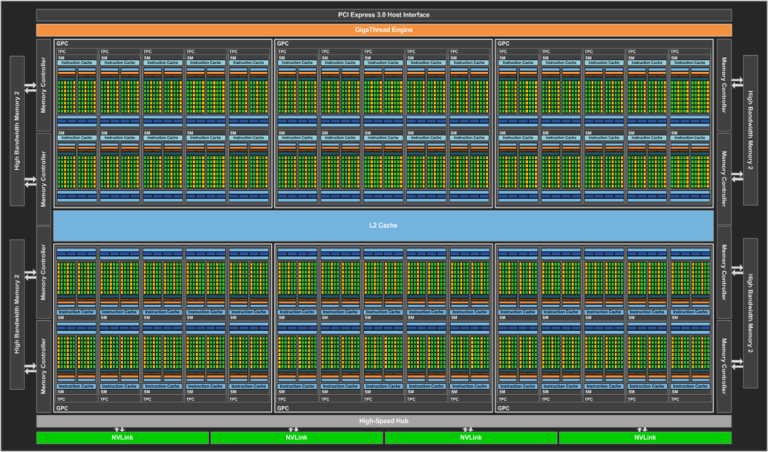
\includegraphics[width=\textwidth]{gpu_pascal}
        \caption[Organization of Cores in NVIDIA Pascal GP100 GPU]{Organization of Cores in NVIDIA Pascal GP100 GPU: In 6 GPCs and 60 SMs, 3840 SP or CUDA Cores (depicted by green blocks) are arranged \cite{ParallelNVIDIA,PascalWhitepaper}.}
        \label{fig:Organization of Cores in NVIDIA Pascal GP100 GPU}
    \end{subfigure}\vspace*{1em}
    \begin{subfigure}{\textwidth}
        \centering
        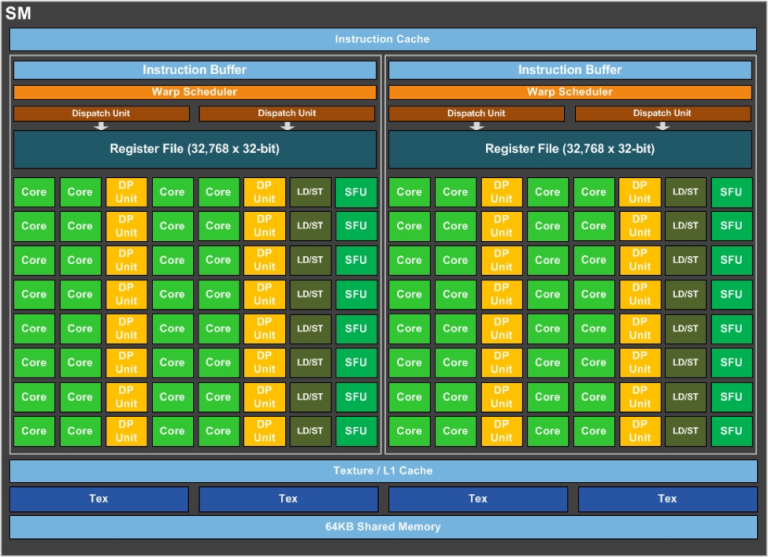
\includegraphics[width=.7\textwidth]{gpu_pascal_sm}
        \caption[Constituents of a Streaming Multiprocessor]{Constituents of a Streaming Multiprocessor \cite{ParallelNVIDIA,PascalWhitepaper}.}
        \label{fig:Constituents of a Streaming Multiprocessor}
    \end{subfigure}
    \caption[The NVIDIA Pascal Architecture]{The NVIDIA Pascal Architecture: A GPU, like a typical CPU, contains multiple hierarchies of memory. In addition, NVIDIA also builds a hierarchy of core organization.}
    \label{fig:The NVIDIA Pascal Architecture}
\end{figure}

The Streaming Multiprocessor (\Cref{fig:Constituents of a Streaming Multiprocessor}), which is the primary multi-threaded multi-processor, houses a shared memory unit for all SPs along with registers and Special Function Units (SFUs), which can calculate specific mathematical functions in fewer clock cycles than threads. The SM is responsible for relaying instructions to threads (in SPs) and maintaining synchronized parallel computation \cite{DemystifyingGPU,PascalWhitepaper}. GPCs and other hierarchies provide abstractions to memory access.

\subsubsection{Memory Organization}
Even the memory units are organized into hierarchies like multi-level caches in CPUs (\Cref{fig:The NVIDIA Pascal Architecture}). In a SM, there are: dedicated local memory units for threads, register files shared by several SPs in a SM, and shared memory caches for all SP Cores in a SM \cite{PascalWhitepaper,ParallelNVIDIA}.

The global internal memory of the GPU (like the RAM of a computer), which is housed separately around the clusters of SMs, stores the complete datasets for a program (when transferred). Data is then distributed in the shared and local memory units once threads start executing an instruction \cite[Appendix~B]{PattersonARM}. Akin the multi-level cache structure in CPUs, this hierarchy of memory enables threads to quickly access working data, thus increasing the performance. Data transfer between the Main Memory of the Scomputer (RAM) and GPU's internal global memory is accomplished with PCI Express lanes \cite{PascalWhitepaper,ParallelNVIDIA}.

\subsubsection{Thread Organization}
According to NVIDIA, the parallel structure is obtained by organizing threads into a hierarchy (``grids'' of ``blocks'' of ``warps'' of ``threads''), where threads of a warp (an abstraction) execute in tandem per clock cycle \cite{CUDADocs,PattersonARM,DemystifyingGPU}. In other words, warps are the basic units of execution in a GPU, which receive single instructions from the controller, and forward them to their constituent threads for execution \cite{CUDADocs,DemystifyingGPU}. This abstraction allows the GPU to execute independent sub-tasks in parallel on a large scale, as shown in \Cref{fig:GPU - Thread Organization in a GPU}.
\begin{figure}[!htbp]
    \centering
    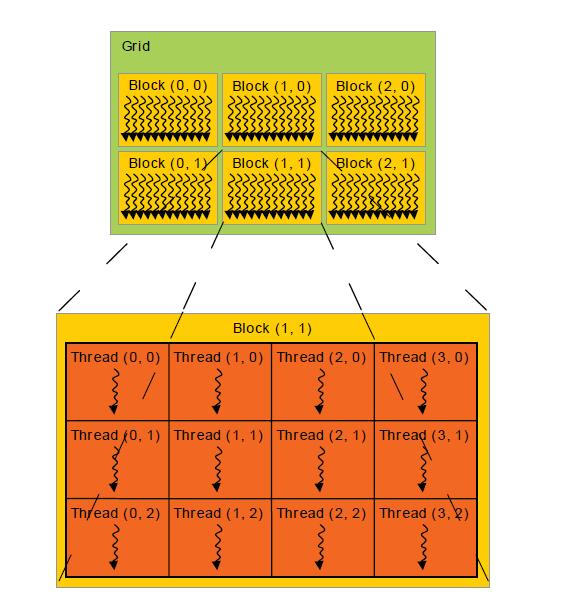
\includegraphics[width=.55\textwidth]{gpu_threads_blocks}
    \caption[Thread Organization in a GPU]{Thread Organization in a GPU: Warps are only an abstraction for identifying threads executing a single instruction; however, threads are physically organized into blocks and grids \cite{CUDADocs,ParallelNVIDIA}}
    \label{fig:GPU - Thread Organization in a GPU}
\end{figure}

NVIDIA calls this setup ``Single-Instruction Multiple-Thread (SIMT)'' \cite{CUDADocs}, where a single instruction is executed in lockstep by multiple threads in a warp (though allowed to branch and diverge). The differences between SIMT and Single-Instruction Multiple-Data (SIMD), a common feature in CPUs, are very subtle. While SIMD distributes data sequences into vectors to be executed by a single core/thread of the CPU (data-level parallelism), SIMT requires a particular thread to only operate on a scalar element of the dataset (thread-level parallelism) \cite{PattersonARM}. In this way, having thousands of threads running in locksteps provides better throughput than vector operations per clock cycle. SIMT also allows programmers to write a program meant for a single, independent thread instead of managing vectors in their code, which promotes ease of use \cite[Chapter~4]{CUDADocs}.

\subsubsection{Instruction Set}
The Instruction Set of a GPU is limited, which causes complex instructions to take several clock cycles. Even though a Special Functional Unit (SFU) computes complex functions (transcendental, reciprocal functions) in fewer clock cycles, their number is small compared to the commonplace threads \cite[Appendix~B]{PattersonARM}. The instruction set for Pascal architecture contains basic operations to load and store memory, perform basic floating point and integer (add, subtract, multiply, divide, min, max etc.) and binary logical operations (or, and, xor, left-shift etc.), and execute jump and branching \cite{DemystifyingGPU,CUDABinUtils}. This comprises a very basic set of instructions unlike those in Intel CPUs, for example, which have coalesced and dedicated architecture for complex instructions\footnote{Intel x86 CPUs have Complex Instruction Set Computing (CISC) Design.} \cite{PattersonARM}.

\subsection{Avoiding Specific Types of Operations in GPUs} \label{sec:Avoiding Specific Operations in GPUs}
GPUs are not better than CPUs at many computations, unlike popular perception. With parallel processing come concerns of synchronization delays, blocking instructions, and program correctness. Moreover, since GPUs are separate units of processors, usually connected to CPUs by PCIe lanes, back and forth memory transfer can cause slowdowns in overall processing performance. Even the GPUs local caches are not big enough to deliver hit rates as compared to CPUs. Often there exists a tradeoff when programming with GPUs, and one should take care to avoid such delays.

\subsubsection{Branch and Diverge}
Since NVIDIA GPUs deal with program correctness through inter-block barrier synchronization (synchronizing after an executed instruction), threads can often go out of sync, blocking the next instruction to execute \cite[Appendix~B]{PattersonARM}. This ultimately causes latency due to synchronization, which can aggregate and slow down the total performance of the program.

To avoid such delays and maximize throughput, one should elude from using extensive branching in the program. In fact, even using small conditional checks can cause a change in a thread's datapath, which can possibly block other threads from proceeding on synchronization barriers. This behavior is aptly termed `branch and diverge' \cite{DemystifyingGPU} \cite[Appendix~B]{PattersonARM}, which occurs when some threads in a warp follow a different datapath due to conditional branching, `diverging' from the group. Now when the warp's threads are forced to converge, those diverging threads would take longer to complete the instruction, causing the non-diverging threads to wait. This radically decreases the throughput of the warp, which again diverges from the block, adding up the latency.
\begin{figure}[!htbp]
    \centering
    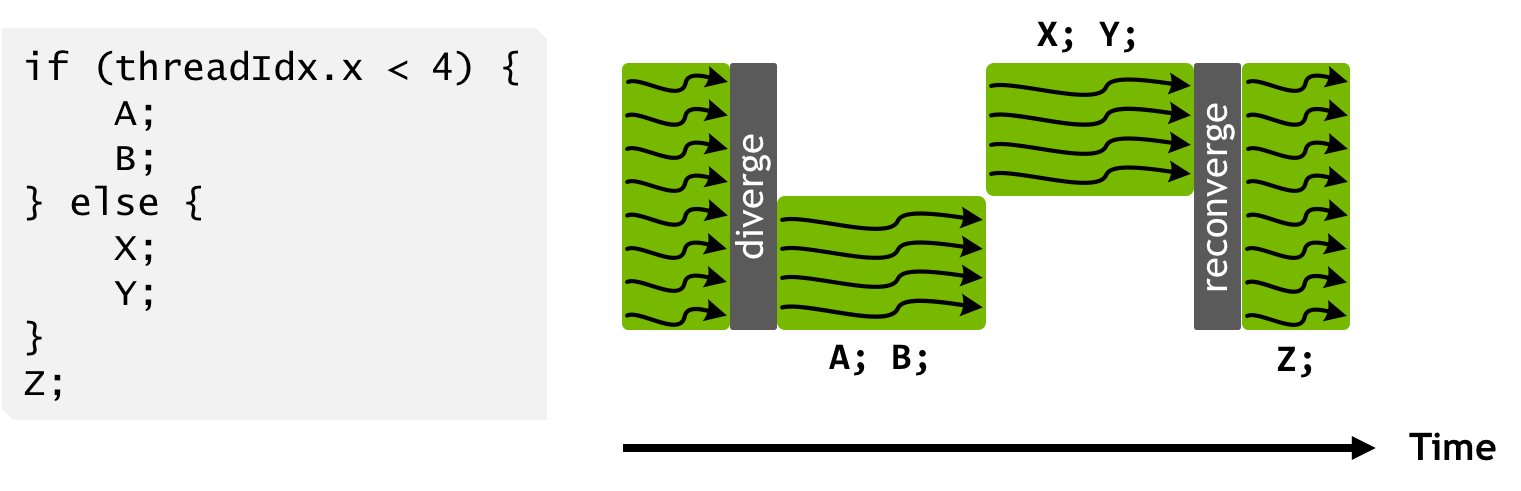
\includegraphics[width=\textwidth]{gpu_branch_diverge}
    \caption[Decrease in GPU Throughput due to Branch and Diverge]{Decrease in GPU Throughput due to Branch and Diverge: In this case, while some threads execute \texttt{A, B}, others execute \texttt{X, Y}. If those sets of operations take unequal time, the threads could diverge from the group and decrease the throughput \cite{ParallelNVIDIA}.}
\end{figure}

\subsubsection{Memory Limitations}
PCIe lanes are not as fast as on-chip CPU cache access or even RAM access times \cite{CUDADocs,ParallelNVIDIA}. As one would expect, transferring datasets back and forth between GPUs and CPUs can add up considerably. Often the limits of GPU's internal memory or required operations on a dedicated device can force the user to transfer datasets multiple times. Even so, one should look for optimizations that can reduce the number of transfers whenever possible, especially when large datasets are involved.

This suggestion is also applicable when transferring datasets in memory intra-GPU (between caches). Miss rates in a GPU's local caches are often high due to limited size, and data requests from higher-level caches can often be expensive.